\chapter{Linear Algebraic Methods}
\label{ch:linalg}

In this chapter we see the first example of a general and flexible
method for bounding the discrepancy of set systems and matrices. The
method is based on linear algebraic arguments, and happens to also
give efficient deterministic algorithms to compute low discrepancy
colorings. It is very versatile, and allows proving non-trivial, and
sometimes even tight bounds in many different settings: we will use it
to bound the discrepancy of set systems with bounded degree, and for systems of
axis-aligned boxes, and of set systems induced by permutations, and to
give bounds for vector balancing and for the Steinitz problem in
arbitrary norms. Some of the ideas developed here will form the basis of
more powerful randomized algorithms presented in later chapters.

\section{The Beck-Fiala Theorem}

Recall that a set system is a pair \((\SS,\uni)\), where $\SS$ is a
collection of subsets of the (finite) universe $\uni$. Let us use the notation
\(\ssdeg(\elem)\) for the degree of \(\elem \in \uni\), i.e., the number
of sets in \(\SS\) that \(\elem\) appears in. The maximum degree
\(\ssdeg(\SS)\) of \(\SS\) is the maximum degree \(\ssdeg(\elem)\) over all
\(\elem \in \uni\). The maximum degree of $\SS$ is a natural measure
of how sparse it is, and we will see that small degree set systems
have a low discrepancy. The next exercise is the easiest interesting
case of this phenomenon.

\begin{exercise}\label{ex:ch2-bf-graphs}
  Given an undirected graph $G = (V,E)$, define $\SS$ with universe $\uni=E$ and  sets $S_u$,
  for each vertex $u \in V$, consisting of all edges with endpoint
  $u$. Then $\ssdeg(\SS) = 2$. Show that if $G$ is
  bipartite, then $\disc(\SS) \le 1$. Show furthermore that $\disc(\SS)
  \le 2$ for all graphs $G$.
\end{exercise}

More generally we have the following fundamental question in
discrepancy theory.
\begin{problem}
  Determine the best possible  bound on the discrepancy \(\disc(\SS)\)
  of a set system $\SS$ as a function of \(\ssdeg(\SS)\).
\end{problem}

In this section, we prove the Beck-Fiala theorem, stated next.
\begin{theorem}\label{thm:ch2-bf}
  For any set system \((\SS, \uni)\) there exists a coloring \(\col\),
  computable in polynomial time, such that \(\disc(\SS,\col) \le 2\ssdeg(\SS)-1\).
\end{theorem}

It should be surprising that
\emph{any} discrepancy bound can be shown purely in terms of $\ssdeg(\SS)$. A key
insight is that a set system with small maximum degree only has few ``large'' sets, i.e., sets of size \(\gg \ssdeg(\SS)\), as we show next.
%This
%follows from counting the number of set-element incidences in two
%ways.
\begin{lemma}\label{lm:ch2-bf-counting}
  For any set system \(\SS\) over a universe $\uni$ of size \(n\), and
  any \(s>0\),   \[
    |\{\set \in \SS: |\set| > s\}| < n\ssdeg(\SS)/s.
  \]
\end{lemma}
\begin{proof}
  Let \(I \eqdef \{(\set, \elem): \elem \in \set\}\) be the set of
  set-element incidences in \(\SS\). We will count \(|I|\) in two
  different ways. On the one hand, $|I| \le n\ssdeg(\SS)$ as each
  element of $\uni$ contributes at most $\ssdeg(\SS)$ incidences. 
  On the other hand, denoting by \(k\) the number of sets in \(\SS\)
  of size greater than \(s\), we have \(|I| > ks\).
  Combining the two inequalities gives \(ks < n\ssdeg(\SS)\), as desired.
\end{proof}

The proof of the Beck-Fiala theorem relies on two observations. The
first is that a set system consisting only of small sets has small
discrepancy. Indeed, \emph{any} coloring of a set of size \(s\) has
discrepancy at most \(s\). The second observation is that requiring that a few sets have small discrepancy still leaves many degrees of freedom for the coloring. In this chapter we formalize this second observation using linear algebra. In Chapter~\ref{ch:partial}, we will see a different formalization through geometry and Gaussian measure, and in Chapter~\ref{ch:partial-alg} we combine the two approaches.

\subsection{The Beck-Fiala Algorithm}
We now prove Theorem \ref{thm:ch2-bf}, using a linear algebraic approach.
%We will present the proof of theorem as an efficient algorithm to compute the coloring $\col$ achieving discrepancy $2\ssdeg(\SS)-1$.

 The key idea that enables using linear algebra is to relax the concept of a coloring to \df{fractional coloring} $\col \in [-1,+1]^\uni$. The algorithm will compute a sequence of fractional colorings $\col_0, \ldots, \col_T$,
 where initially, $\col_0$ assigns color $0$ to every element, and at each step $t$, $\col_t$ colors at least one more element with $\pm 1$ than $\col_{t-1}$. So by step $T \le n$, $\col_T \in \{-1,+1\}^\uni$.
 
 Whenever some color $\col_t(\elem)$ reaches $\{-1,+1\}$, we fix $\col_t(\elem)$ forever, and we also maintain the invariant that $\col_t(S) = \col_{t-1}(S)$ for all sets $S \in \SS$ that have more than $\ssdeg(\SS)$ elements that are not yet colored $\pm 1$. These are the ``dangerous sets'' -- with potential to incur large discrepancy. %All other sets are safe, since their discrepancy can change by at most $2\ssdeg(\SS)$ no matter how the not yet fixed elements are colored. 
 The existence of such $\col_t$ will follow from Lemma~\ref{lm:ch2-bf-counting} and a simple linear algebraic argument.

%intuition, however, is tricky. The approach we take in this chapter, and in much of the rest of the book, is to
% relax the concept of a coloring to a \df{fractional coloring}, where
% elements can be colored by real numbers in \([-1,+1]\). To make a
% fractional coloring useful, we also require that some number of
% elements are properly colored, i.e., they are colored with \(+1\) or
% \(-1\). Such colorings can be combined to yield a coloring where each
% element's color is in \(\{+1,-1\}\). At the same time, allowing
% fractional colors makes it possible to use tools from continuous
% mathematics, \eg linear algebra, to show the existence of a good
% coloring.

% The next lemma
% is an illustration of this approach.

% \begin{lemma}\label{lm:ch2-bflemma}
%   Let \((\SS, \uni)\) be a set system, let \(\col_0:\uni \to [-1,+1]\) be a
%   fractional coloring, and let
%   \(\act \subseteq \uni\) be such that, for any \(\elem \in \act\),
%   \(|\col_0(\elem)| < 1\). If \(|\SS| < |\act|\), then there exists another
%   fractional coloring \(\col:\uni \to [-1,+1]\) such that
%   \begin{enumerate}
%   \item for all \(\set \in \SS\), \(\col(\set) = \col_0(\set)\);\label{item:ch2-bflemma-1}
%   \item for all \(\elem \in \uni\setminus\act\), \(\col(\elem) = \col_0(\elem)\);\label{item:ch2-bflemma-2}
%   \item there exists some \(\elem \in \act\) such that
%     \(\col(\elem) \in \{-1,+1\}\).\label{item:ch2-bflemma-3}
%   \end{enumerate}
%   Moverover, given \(\SS\) and \(\col_0\), \(\col\) can be computed in
%   polynomial time.
% \end{lemma}

% If we take \(\col_0(\elem) = 0\) for every \(\elem \in \uni\), then
% Lemma~\ref{lm:ch2-bflemma} gives a coloring with discrepancy 0 that
% properly colors at least one element. While this fact is not that
% interesting by itself, the lemma proves more: it
% shows that, for a set system with sufficiently few sets, any fractional
% coloring can be extending by properly coloring at least one more
% element, while not affecting the discrepancy of the sets. This is
% very useful in building a proper coloring out of a fractional one.

% Lemma~\ref{lm:ch2-bflemma} is a consequence of the following linear
% algebraic statement.

% \begin{lemma}\label{lm:ch2-bflinalg}
%   Let \(\mat\) be an \(m \times n\) matrix such that
%   \(\rank \mat < n\), and let \(\col_0 \in (-1,+1)^n\). Then there exists
%   some \(\col \in [-1,+1]^n\) such that \(\mat \col = \mat \col_0\), and
%   \ for some \(i \in [n]\) we have \(\col(i) \in
%   \{-1,+1\}\). Moreover, \(\col\) can be computed in polynomial time given
%   \(\mat\) and \(\col_0\).
% \end{lemma}
% \begin{proof}
%   Since \(\rank \mat < n\), the columns of \(\mat\) are
%   linearly dependent, so there exists some \emph{nonzero} \(\Delta \col \in \R^n\) for
%   which \(\mat \Delta \col = 0\). To get \(\col\) from \(\col_0\), we
%   move from \(\col_0\) in the direction of \(\Delta \col\) until we
%   hit the boundary of the cube \([-1, +1]^n\), as shown in
%   Figure~\ref{fig:ch2-bflemma}. In other words, we choose \(t > 0\) to be the largest real number
%   such that \(\col_0 + t\Delta\col \in [-1, +1]^n\), and set \(\col =
%   \col_0 + t\Delta\col\). Then, since \(\mat \Delta \col = 0\),
%   \[
%     \mat\col = \mat \col_0 + t\mat \Delta \col = \mat \col_0,
%   \]
%   and, furthermore, there must be some \(i\in [n]\) for which
%   \(\col(i) \in \{-1,+1\}\), or, otherwise, \(t\) could be chosen
%   larger.
%   \begin{figure}[htp]
%     \centering
%     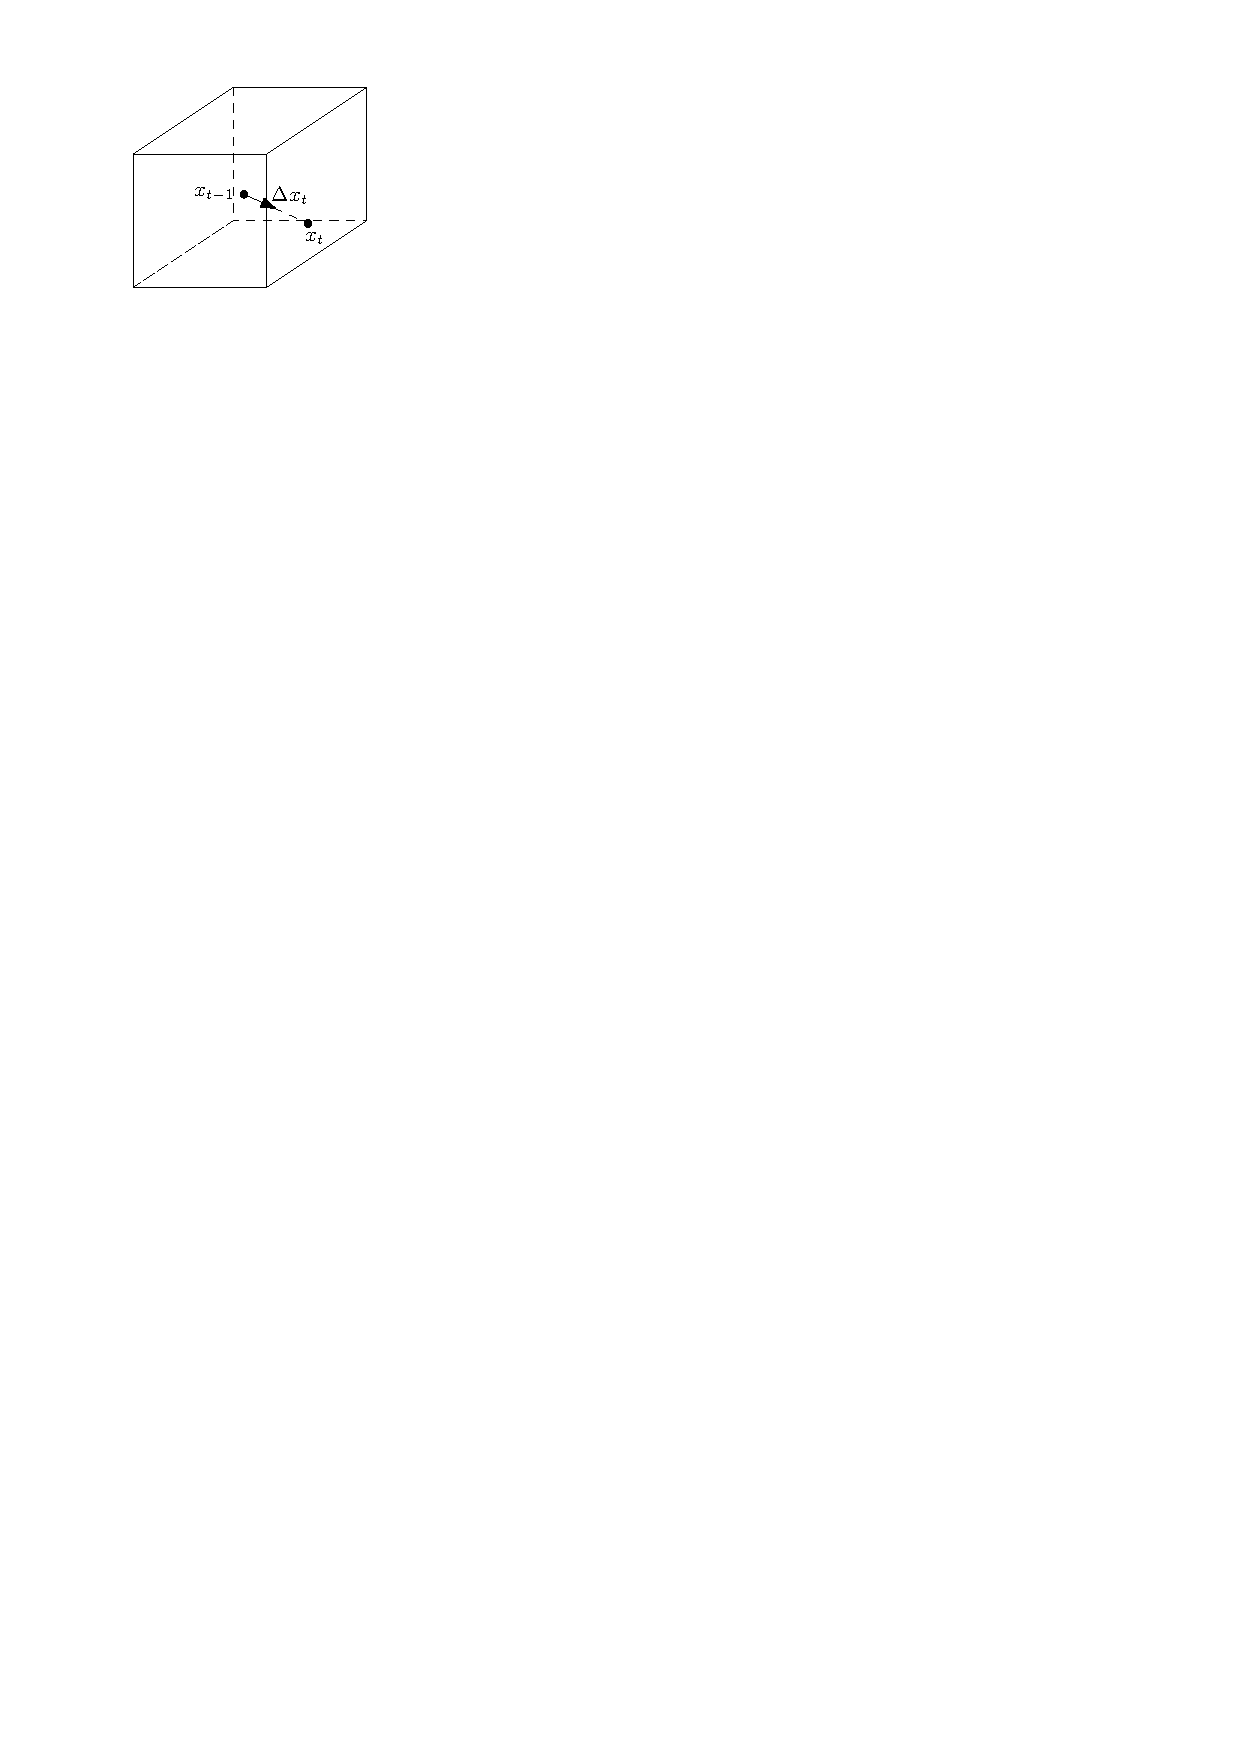
\includegraphics{bflemma}
%     \caption{We find \(\col\) by starting from \(\col_0\) and going in
%       the direction of \(\Delta \col\) until we hit a boundary of the
%       cube \([-1, +1]^n\).}
%     \label{fig:ch2-bflemma}
%   \end{figure}

%   To compute \(\col\), we need to compute \(\Delta\col\) and
%   \(t\). To compute \(\Delta\col\), we need to find a nonzero vector
%   in the nullspace of \(\mat\), which can be done efficiently via
%   Gaussian elimination. Then \(t\) can be computed by the formula
%   \[
%     t =
%     \min\left\{\frac{\sign(\Delta\col(i))-\col_0(i)}{\Delta\col(i)}:
%       \Delta\col(i) \neq 0\right\}
%   \]
%   where \(\sign(x)\) is \(+1\) for positive \(x\), and \(-1\) for
%   negative \(x\).
% \end{proof}

% We can now deduce Lemma~\ref{lm:ch2-bflemma} from
% Lemma~\ref{lm:ch2-bflinalg}.

% \begin{proof}[Proof of Lemma~\ref{lm:ch2-bflemma}]
%   We let \(\mat\) be the incidence matrix of \(\SS|_{\act}\), i.e., the matrix with rows indexed by \(\SS\), and
%   columns indexed by \(\act\), and with entries
%   \[
%     \matent(\set,\elem) \eqdef
%     \begin{cases}
%       1 & \elem \in \set\\
%       0 & \elem \not \in \set
%     \end{cases}.
%   \]
%   Then \(\rank \mat \le |\SS| < |\act|\) by
%   assumption, and we can apply Lemma~\ref{lm:ch2-bflinalg} to \(\mat\)
%   and to \(\col_0\) restricted to \(\act\). We extend
%   the fractional coloring \(\col\) of \(\act\)
%   guaranteed by Lemma~\ref{lm:ch2-bflinalg} to a coloring of \(\uni\)
%   so that it agrees with \(\col_0\) on \(\uni\setminus\act\); thus, condition
%   \ref{item:ch2-bflemma-2}.~is satisfied by construction. Conditions
%   \ref{item:ch2-bflemma-1}.~and \ref{item:ch2-bflemma-3}.~follow from the conclusion of Lemma~\ref{lm:ch2-bflinalg}.
% \end{proof}

% We are now ready to prove the Beck-Fiala theorem. In the proof, we repeatedly use
% Lemma~\ref{lm:ch2-bflemma} to update a fractional coloring until it
% becomes a proper coloring.

% \begin{algorithm}
%   \begin{algorithmic}
%     % \Procedure{Beck-Fiala}{\(\SS, \uni\)}
%     \Require Set system \((\SS, \uni)\), \(n = |\uni|\);
%     \Ensure Coloring \(\col\) such that \(\disc(\SS, \col) \le
%     2\ssdeg(\SS) - 1\);
%     \State Initialize \(\col_0 = 0, \act_0 = \uni\);
%     \For{\(t = 1\ldots n\)}
%        \State \(\DD_t = \{\set \in \SS:  |S\cap \act_{t-1}| >  \ssdeg(\SS)\}\);
%        \State Apply Lemma~\ref{lm:ch2-bflemma} to the set system
%        \((\DD_t,\uni)\), the coloring \(\col_{t-1}\), and the set \(\act_{t-1}\), to get a new
%        coloring \(\col_t\) s.t.~
%        \begin{enumerate}
%        \item for all \(\set \in \DD_t\), \(\col_t(\set) = \col_{t-1}(\set)\);
%        \item for all \(\elem \in \uni\setminus\act_{t-1}\), \(\col_t(\elem) = \col_{t-1}(\elem)\);
%        \item there exists some \(\elem \in \act_{t-1}\) such that
%          \(\col_t(\elem) \in \{-1,+1\}\);
%        \end{enumerate}
%        \State \(\act_t = \{\elem \in \uni: |\col_t(\elem)| < 1\}\);
%        \If{\(\act_{t} = \emptyset\)}
%           \State Exit loop and return \(\col = \col_{t}\);
%        \EndIf
%        \EndFor
%        \State Return \(\col = \col_n\).
%     %\EndProcedure
%   \end{algorithmic}
%   \caption{The Beck-Fiala Algorithm}
%   \label{alg:beck-fiala}
% \end{algorithm}

\paragraph{The Formal Algorithm.} The coloring \(\col\) is computed by an iterative algorithm. At each step \(t\), the algorithm maintains a fractional coloring \(\col_t \in [-1,1]^\uni\), a set of fixed elements \(F_t \eqdef \{\elem \in \uni: |\col_{t-1}(\elem)| = 1\}\), and a set of ``dangerous'' sets \(\DD_t \eqdef \{\set \in \SS:|\set \setminus F_t| > \ssdeg(\SS)\}\). 
Initially, we set \(\col_0 \eqdef 0\), and the algorithm terminates when \(F_{t+1} = \uni\), at which point we output \(\col \eqdef \col_t\). 

To compute $\col_t$ from $\col_{t-1}$, in step \(t \ge 1\), we find a nonzero update vector $\Delta\col_t$ such that 
\begin{enumerate}
\item \(\Delta\col_t(\set) := \sum_{\elem \in \set}\Delta\col_t(\elem) = 0\) for all dangerous sets \(\set \in \DD_t\);\label{enum:bf-dangerous}
\item $\Delta\col_t(\elem) = 0$ for all fixed elements \(\elem \in F_t\).\label{enum:bf-fixed}
\end{enumerate}
We argue why such a $\Delta\col_t$ exists below. To compute the coloring $\col_t$, we set $\col_t = \col_{t-1} + \gamma \Delta \col_t$, where we choose $\gamma > 0$ to be the largest possible value such that $\col_t \in [-1,1]^\uni$. See Figure~\ref{fig:ch2-bflemma}. 

\begin{figure}[htp]
\centering
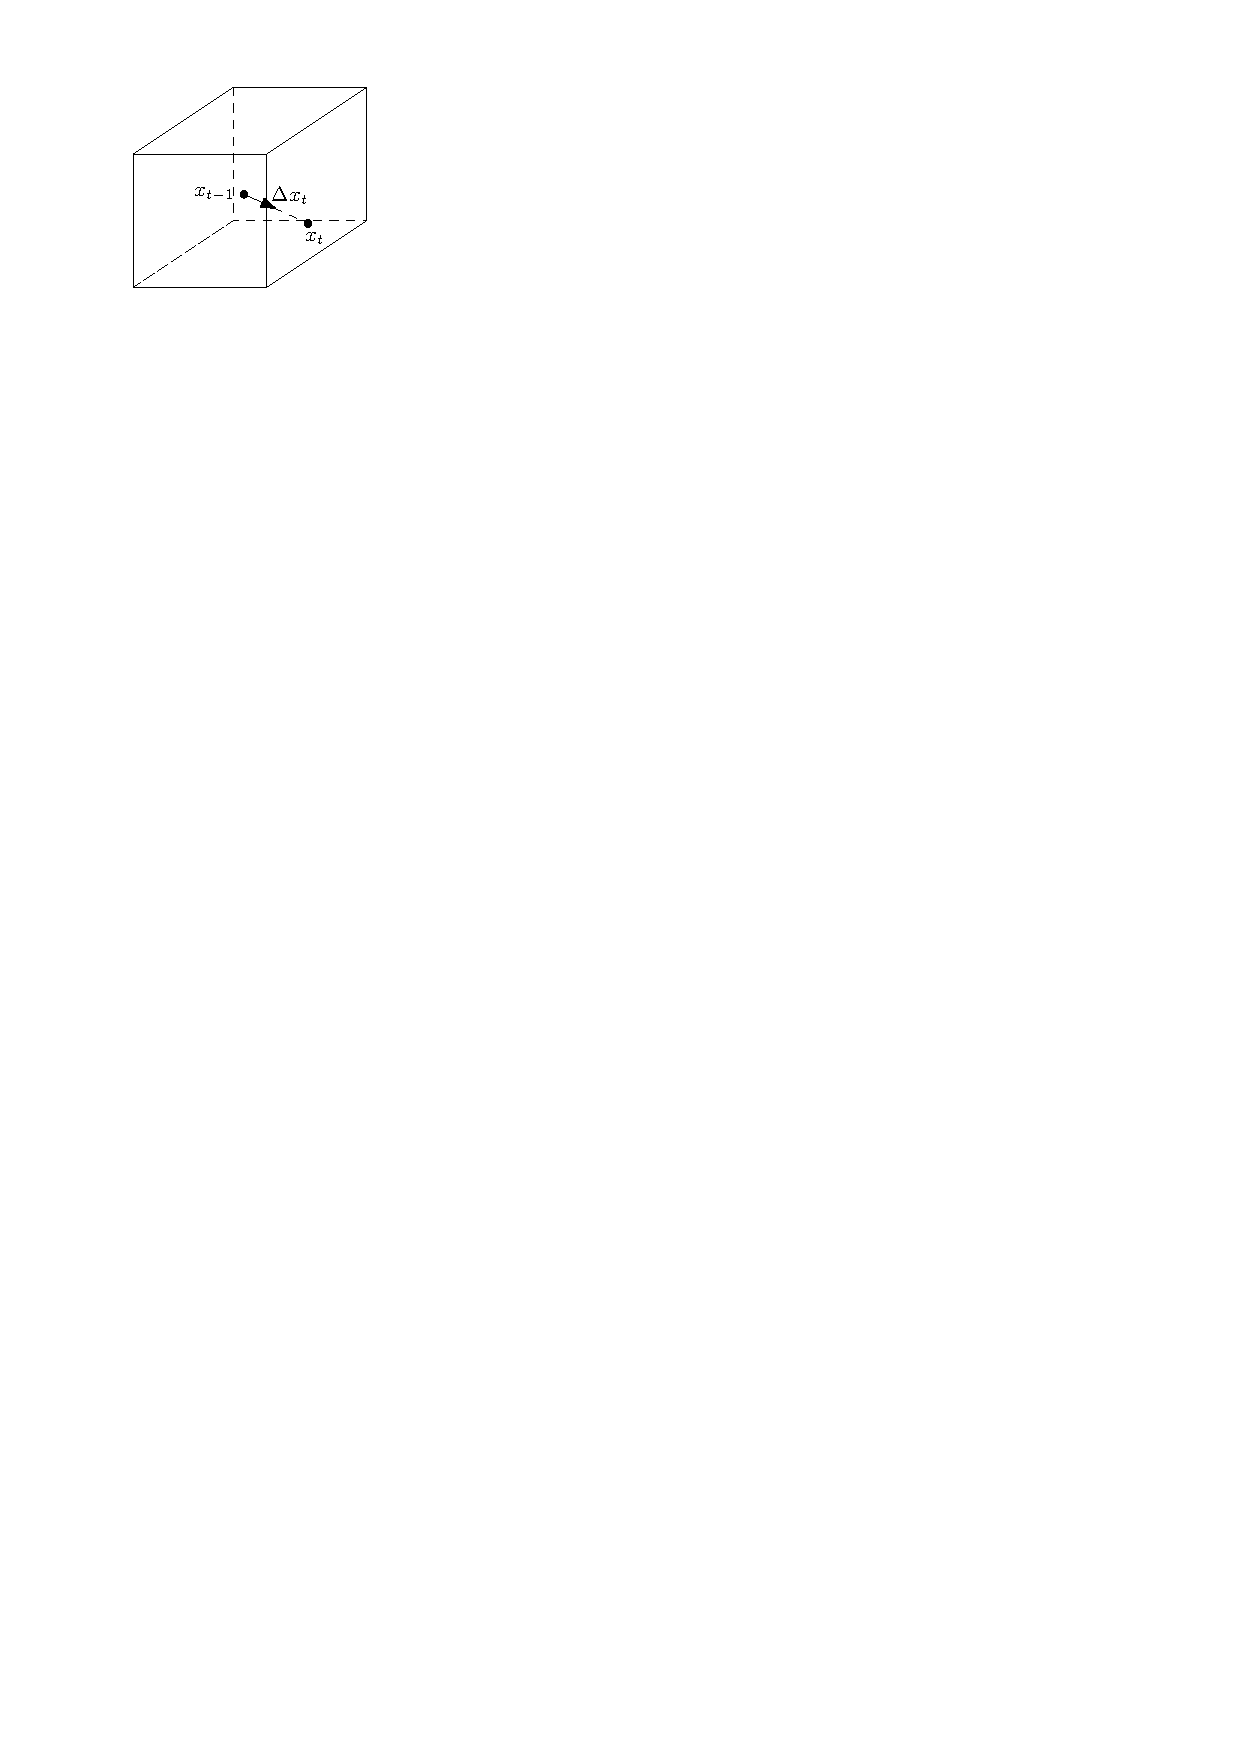
\includegraphics{bflemma}
\caption{We find \(\col_t\) by starting from \(\col_{t-1}\) and going in the direction of \(\Delta \col_t\) until we hit a boundary of the cube \([-1, +1]^\uni\).}
\label{fig:ch2-bflemma}
\end{figure}


\paragraph{Analysis.} Let us use the notation $\act_t \eqdef \uni \setminus F_t$ for the ``active'' elements, i.e., the ones not yet fixed. First we verify that, as long as $F_t \neq \uni$ (equivalently $\act_t \neq \emptyset$), there exists a $\Delta\col_t \neq 0$ satisfying \ref{enum:bf-dangerous}.~and~\ref{enum:bf-fixed}. The two conditions form a system of linear equations, and to show that the system has a nonzero solution $\Delta\col_t$, we will argue that it is under-constrained. By Lemma~\ref{lm:ch2-bf-counting}, applied to the set system \(\SS|_{\act_{t}}\) with \(s = \ssdeg(\SS) \ge \ssdeg(\SS|_{\act_{t}})\), we have that \(|\DD_t| < |\act_{t}|\). Thus, $\Delta \col_t$ must satisfy at most $|\DD_t| + |F_t| = |\DD_t| + (n-|\act_{t}|) < n$ linear equations, and the subspace of solutions to these equations has dimension at least $1$. This shows that we can find some $\Delta \col_t \neq 0$ satisfying \ref{enum:bf-dangerous}.~and~\ref{enum:bf-fixed}.

Next, the algorithm terminates in at most $n$ steps as $F_{t+1} \supsetneq F_{t}$, by the choice of $\gamma$ and thus $|F_t|$ increases by at least $1$ in each step. 

Finally, we analyze the discrepancy of the final coloring $\col = \col_T$. Notice that, as $F_t$ is increasing in $t$, \(\DD_{t} \subseteq \DD_{t-1}\), i.e., a set can only stop being dangerous once, and it never becomes dangerous again. Since initially $\col_0(S) = 0$ for all $S \in \SS$, we have that \(\col_t(\set) = 0\) as long as \(\set \in \DD_t\). 
To bound the final discrepancy, consider an arbitrary set \(\set \in \SS\), and suppose that it was last dangerous at time step \(t=t(S)\), i.e., \(\set \in \DD_{t} \setminus \DD_{t+1}\). Then,
\[
    |\col(\set)| \le |\col_{t}(\set)| + |\col(\set) - \col_{t}(\set)|
    = |\col(\set) - \col_{t}(\set)|.
\]
As the color stays unchanged for any element \(\elem \in F_{t+1}\) after time $t$, we have \(\col(\elem) = \col_t(\elem)\) and thus 
\begin{align*}
    & |\col(\set) - \col_{t}(\set)|
    =
    \Big|\sum_{\elem \in \set \setminus F_{t+1}} (\col(\elem) -  \col_t(\elem))\Big|\\
    &\le \sum_{\elem \in \set \setminus F_{t+1}} |\col(\elem) -  \col_t(\elem)| < 2|\set \setminus F_{t+1}| \le 2 \ssdeg(\SS).
\end{align*}
The strict inequality follows since \(\col(\elem) \in \{-1,+1\}\), and \(\col_t(\elem) \in (-1, +1)\) for any \(\elem \not\in F_{t+1}\), thus \(\col(\elem) - \col_t(\elem) \in (-2, 2)\). The final inequality follows as \(\set \not \in \DD_{t+1}\). 

We have now shown that \(|\col(\set)| < 2 \ssdeg(\SS)\), and, as \(|\col(\set)|\) is an integer,  we must have \(|\col(\set)| \le 2 \ssdeg(\SS)-1\). As \(\set\) was arbitrary, the result follows.


\paragraph{Improvements.} Theorem~\ref{thm:ch2-bf} is not tight, and Beck and Fiala
conjectured that the tight bound is \(\disc(\SS) \lesssim
\sqrt{\ssdeg(\SS)}\). The best known bounds (for general \(\ssdeg(\SS)\))  that only depend on
\(\ssdeg(\SS)\) are linear in \(\ssdeg(\SS)\), and, in fact, even the leading
constant \(2\) has not been improved.\footnote{Very recently, Bansal and Jiang \cite{bansaljiang2025} proved the conjectured $O(\sqrt{\ssdeg(\SS)})$ bound when $\ssdeg(\SS) = \Omega(\log^2 n)$.} Later in this book we will see
bounds that have only mild dependence on the number of elements
\(n\). 

For now, the next exercise gives a small improvement to
Theorem~\ref{thm:ch2-bf}.

\begin{exercise}\label{ex:ch2-bf-improvement}
  Modify the proof of Theorem~\ref{thm:ch2-bf} to show the improved
  bound $\disc(\SS) \le \max\{2\ssdeg(\SS) - 3, \ssdeg(\SS)\}$.

  \textsc{Hint:} By an argument analogous to
  Lemma~\ref{lm:ch2-bf-counting}, a set system on $n$ elements with maximum degree $s$
  has at most $n$ sets with size at least $s$. What happens when the
  set system has exactly $n$ such sets?
\end{exercise}

Note that, unlike Theorem~\ref{thm:ch2-bf},
Exercise~\ref{ex:ch2-bf-improvement} recovers the (tight) bound
$\disc(\SS) \le 2$ when $\ssdeg(\SS) \le 2$. 

\section{Template of a Linear Algebraic Algorithm}

In this section we generalize the approach taken in the proof of the Beck-Fiala theorem to formulate a template for an algorithm computing low discrepancy colorings using linear algebra. We will use it later for various applications. We keep the notation from the proof of Theorem~\ref{thm:ch2-bf} whenever possible.

\paragraph{The Generic Algorithm.} We start with
some fractional coloring $\col_0 \in [-1,1]^n$, usually
$\col_0 \eqdef 0.$ Then we construct a coloring in \emph{phases}, where in the $t$-th phase we compute $\col_t$. 

In phase $t$, we define a matrix $\mat_t$ of \emph{dangerous directions}, and a set of \emph{active} elements $\act_t \subseteq [n]$. The set of \emph{fixed} elements is always $F_t \eqdef \{i \in [n]: |\col_{t-1}(i)| = 1\}$, and we require $\act_t \cap F_t = \emptyset$. We choose the next coloring $\col_t$ so that
\begin{enumerate}
    \item $\mat_t\col_t = \mat_t \col_{t-1}$;
    \item $\col_t(i) = \col_{t-1}(i)$ for each
$i \not \in \act_{t}$.
\end{enumerate}
We also aim to fix as many elements as possible, i.e., to maximize $|F_{t+1}| - |F_t|$. At the first $T$ for which $F_{T+1} = [n]$, we output $\col_T$.

Intuitively, each row of $\mat_t$ defines a ``dangerous direction'', and moving the coloring in such a direction may incur too much discrepancy. For this reason we ask the coloring update $\Delta x_t = x_t - x_{t-1}$ to lie in the kernel of $\mat_t$, which is our ``safe subspace''.  

The proof of the Beck-Fiala theorem follows the template above. In it, each phase fixes the color of at least one element, leading up to $n$ phases. In other applications, we may want to fix more elements in a single phase so that the number of phases becomes much smaller. To compute $\col_t$ from $\col_{t-1}$ we shall use the following lemma. 

Recall that \(\mat(*, J)\) denotes the submatrix of \(\mat\) consisting of the columns indexed by the set \(J\).

\begin{lemma}\label{lm:ch2-linalg-gen}
  Let \(\mat\) be an \(m \times n\) matrix, let \(\col \in
  [-1,+1]^n\), and let \(\act \subseteq [n]\) be such that for any \(i
  \in \act\), \(|\col(i)| < 1\).  If \(\rank \mat(*,\act) <
  |\act|\), then there exists a \(\col' \in [-1,
  +1]^n\) such that
  \begin{enumerate}
  \item \(\mat \col' = \mat \col\);
  \item for any \(i \in [n] \setminus \act\), \(\col'(i) = \col(i)\)
  \item for at least \(|\act| - \rank \mat(*,\act)\) elements 
    \(i \in \act\), we have \(\col'(i) \in \{-1, +1\}\).
  \end{enumerate}
  Moreover, given \(\mat\) and \(\col\), \(\col'\) can be computed in
  polynomial time.
\end{lemma}
% \begin{proof}
%   We repeatedly find a good direction in which to update $\col$. 
%   We set $\col_0 \eqdef \col$, and \(\act_0 \eqdef  \act\), and, at step \(t\) we compute \(\col_t\in [-1,+1]^n\) such that
%   \begin{enumerate}
%   \item \(\mat \col_t = \mat \col_{t-1}\);
%   \item for all \(i \in [n]\setminus\act_{t-1}\), \(\col_t(i) = \col_{t-1}(i)\);
%   \item for some  \(i \in \act_{t-1}\) we have  \(\col_{t}(i) \in \{-1,+1\}\).
%   \end{enumerate}
%   We terminate when \(\rank \mat(*,\act_{t}) = |\act_t|\). 
%   Notice that, before we terminate, the system of
%   homogeneous linear equations
%   $\mat \Delta \col_t = 0$ and $\Delta \col_t(i)= 0$ for all $i \not \in
%   \act_{t-1}$ has rank at most
%   \[
%     n-|\act_{t-1}| + \rank  \mat(*,\act_{t-1}) < n,
%   \]
%   and therefore, this system has a nonzero solution. We then compute
%   $\col_t \eqdef \col_{t-1} + \gamma \Delta\col_t$ where $\gamma > 0$
%   is chosen to be the largest value for which $\col_t \in
%   [-1,+1]^n$. It is easy to verify that this $\col_t$ satisfies the
%   conditions above and can be computed efficiently.

%   Since \(|\act_{t}| < |\act_{t-1}|\), it is clear that the algorithm
%   will terminate in at most \(|\act| \le n\) steps.
%   Suppose \(T\) is
%   the first time step when \(\rank \mat(*,\act_{T}) = |\act_T|\), and
%   set \(\col' \eqdef \col_T\). Then
%   the number of elements \(i \in \act\) such that \(\col'(i) \in \{-1,
%   +1\}\) is equal to 
%   \[
%     |\act| - |\act_T| = |\act| - \rank \mat(*,\act_{T}) \ge |\act| -
%     \rank \mat(*,\act),
%   \]
%   since \(\act_t \subseteq \act\) for any \(t\). The other two
%   properties of \(\col'\) follow by a straightforward induction
%   on \(t\).
% \end{proof}

The proof of Lemma~\ref{lm:ch2-linalg-gen} is simple and left as an exercise.

Similar to the proof of the Beck-Fiala theorem, we start initially with $\col_0= 0^n$ and iteratively update the coloring $\col_t$ to $\col_{t+1}= \col_t + \Delta \col_t$ at each step using Lemma~\ref{lm:ch2-linalg-gen} with $x=\col_t$ and $x'=\col_{t+1}$.

% find update directions $\Delta\col_t = x'-\neq 0$ such that $\mat\Delta\col = 0$ and $\Delta\col(i) = 0$ for all $i$ that have reached $-1$ or $+1$. Whenever such a $\Delta \col$ exists, we update $\col'$ to $\col' + \gamma \Delta\col$ for $\gamma$ as large as possible so that $\col'$ stays in $[-1,1]^n$. We terminate when there does not exist an update direction.

One may wonder if we can gain something by picking the update $\Delta \col_t$ more carefully. In Chapter~\ref{ch:partial-alg} we will see an example of this, where the directions are picked randomly from some appropriate distribution.

Applying Lemma~\ref{lm:ch2-linalg-gen}  to the incidence matrix of
a set system gives the following immediate corollary that we record for ease of reference.
%\sasho{This is used once, so may not
%  be worth stating it?}

\begin{lemma}\label{lm:ch2-fewsets}
  Let \((\SS, \uni)\) be a set system, let \(\col\in [-1,+1]^\uni\) be a
  fractional coloring, and let
  \(\act \subseteq \uni\) be the set of elements with \(|\col(\elem)| < 1\). If \(|\SS|_{\act}| < |\act|\), then there is a \(\col' \in [-1,+1]^\uni\) such that
  \begin{enumerate}
  \item for all \(\set \in \SS\), \(\col'(\set) = \col(\set)\);%\label{item:ch2-bflemma-1}
  \item for all \(\elem \in \uni\setminus\act\), \(\col'(\elem) = \col(\elem)\);%\label{item:ch2-bflemma-2}
  \item for at least \(|\act|-|\SS_{|\act}|\) elements \(\elem \in
    \act\) we have
    \(\col'(\elem) \in \{-1,+1\}\).%\label{item:ch2-bflemma-3}
  \end{enumerate}
  Moreover, given \(\SS\) and \(\col\), \(\col'\) can be computed in
  polynomial time.
\end{lemma}

\paragraph{Simple Application.} As an application of Lemma~\ref{lm:ch2-linalg-gen}, we first show
a useful structural result about discrepancy, that the
hereditary discrepancy of any \(m\times n\) matrix is always achieved, up to a
factor of \(2\), on a submatrix consisting of at most \(m\) columns
from \(\mat\). For this reason, discrepancy bounds in terms of \(n\)
can often be automatically strengthened to hold in terms of
\(\min\{m,n\}\) instead.

\begin{theorem}\label{thm:ch2-col-reduction}
  Let \(\|\cdot\|_X\) be a norm on \(\R^m\), and let \(\mat\) be an
  \(m\times n\) matrix. Then there exists a set \(J \subseteq [n]\) of
  size \(|J| \le m\) such that
  \[
    \disc_X(\mat) \le %\lindisc_X(\mat(*,J)) 
     2 \herdisc_X(\mat(*,J)) \le 2\herdisc_X(\mat,m)
  \]
%  Moreover, on input \(\mat\), \(J\) can be computed in polynomial time. When given oracle access to an algorithm that, on input \(\mat(*,J)\) and some \(y \in [-1, 1]^J\), computes a \(\col \in \{-1, +1\}^J\) satisfying \(\|\mat(*,J)(\col-y)\|_X \le D\), a coloring \(\col' \in \{-1, +1\}^n\) for which \(\|\mat\col'\|_X \le D\) can also be computed in polynomial time.
\end{theorem}
\begin{proof}
  We apply Lemma~\ref{lm:ch2-linalg-gen} with the matrix \(\mat\),
  \(\act = [n]\), and \(\col = 0\). This gives us a fractional
  coloring \(\col'\) for which \(\mat \col' = 0\), and the set
  \(J \eqdef \{i: |\col'(i)| < 1\}\) has size at most
  \(\rank \mat \le m\). 
  Let \(y\in [-1,+1]^J\) be \(\col'\)
  restricted to \(J\). 
  By Theorem~\ref{thm:ch1-transference}, there
  exists some coloring \(z \in \{-1,+1\}^J\) such that
  \(\|\mat(*,J)(z-y)\|_X \le 2\herdisc_X(\mat(*,J))\). 
  
  We can then
  extend \(\col'\) to a coloring \(\col''\in \{-1,+1\}^n\) by setting
  \[
    \col''(i) \eqdef
    \begin{cases}
      z(i) & i \in J\\
      \col'(i) & i \not \in J. 
    \end{cases} %\qedhere
  \]
  We now have
  \[
  \disc_X(\mat,\col'') 
  \le
  \|\mat \col'\|_X + \|\mat(*,J)(z-y)\|_X = 2\herdisc_X(\mat(*,J)),
  \]
  as we needed to show.
%  The second inequality follows from~\sasho{add ref to LSV
 %   rounding theorem here}.
%\nikhil{fix this later. just commented it out}
\end{proof}


\section{Discrepancy of Permutations}

For our next application of the linear algebraic method, we study the
discrepancy of set systems consisting of prefixes of \(k\)
permutations. We are given \(k\) permutations \(\pi_1, \ldots, \pi_k\)
of \([n]\), and the set system \((\SS, [n])\) consists of prefixes of
the permutations, i.e., all sets of
the form \(\{\pi_i(1), \ldots, \pi_i(j)\}\) where \(i\) and \(j\)
range over \([k]\) and \([n]\), respectively. We say that \(\SS\)
is the set system induced by \(\pi_1, \ldots, \pi_k\). One of the
problems we will return to later in the book is determining the
discrepancy of such set systems.
\begin{problem}
  For a set system \((\SS, [n])\) induced by \(k\) permutations of
  \([n]\), determine the best possible bound on \(\disc(\SS)\) as a
  function of \(n\) and \(k\).
\end{problem}
In addition to being
natural set systems in their own right, \(k\) permutation systems are
useful when studying the discrepancy of rectangles, and they have 
applications to approximation algorithms. We will see the first connection later in this chapter. 

The discrepancy of set systems induced by \(k\) permutations exhibits
an interesting transition: it is equal to \(1\) when \(k\) is \(1\) or
\(2\), and can be as large as \(\Omega(\log n)\) for any \(k\ge
3\). When \(k = 1\), we can just color \(\pi(1), \ldots,
\pi(n)\) with alternating colors, in this order, and the resulting
coloring clearly has discrepancy \(1\). 

\medskip 
%\noindent{\bf Two Permutations.} 
The case of \(2\) permutations
is more interesting, and we briefly sketch the construction of a
coloring \(\col\) with discrepancy \(1\). The idea is to ensure, for
every \(i \in [2]\), and \(j \in [\lfloor n/2\rfloor]\) that
\(\col(\pi_i(2j - 1)) \neq \col(\pi_i(2j))\). Then, any prefix
\(\set\) of either permutation can be partitioned into the pairs \(\{\pi_i(2j-1),
\pi_i(2j)\}\), and at most one additional element, and each pair
contributes discrepancy \(0\) to \(\col(\set)\).

To find such a coloring \(\col\) we construct a graph \(G = ([n], E)\), where the
edge set \(E\) consists of all such pairs \(\{\pi_i(2j-1),
\pi_i(2j)\}\).
Then, the coloring \(\col\) that we
need corresponds to a proper 2-coloring of the vertices of \(G\),
which exists as \(G\) is a union of two
matchings, and hence a disjoint union of paths and even length
cycles.


% Therefore, \(G\) is a bipartite graph and can be properly
% \(2\)-colored.

\paragraph{$k$ Permutations.}
The combinatorial argument above does not extend to \(3\) or more
permutations, but the linear algebraic method allows us to prove an \(O(k \log n)\) bound on the discrepancy of \(k\)
permutations. 

The idea is to divide the permutations into intervals, and
make sure that each interval receives zero total discrepancy, but with respect to a fractional coloring, rather than a full \(\pm 1\)
coloring. In order to find such a fractional coloring using
Lemma~\ref{lm:ch2-fewsets}, we need that the total number of intervals whose discrepancy we keep at \(0\) is small. In particular, we make sure that the number of intervals is at most half the number of active elements, and thus we can fix half of them in each phase. This guarantees we can find a proper coloring in $O(\log n)$ phases, giving the logarithmic discrepancy bound. 

Formally, we show the following.

\begin{theorem}\label{thm:ch2-kperm}
  For any integers \(k \ge 1\) and \(n\ge 1\), and any permutations \(\pi_1,
  \ldots, \pi_k\) of \([n]\), there exists a coloring \(\col\),
  computable in polynomial time, such that for the set system \((\SS,
  [n])\) induced by \(\pi_1, \ldots, \pi_k\) we have
  \(
  \disc(\SS) \lesssim k \log 2n.
  \)
\end{theorem}

\paragraph{The Algorithm.} We apply our template. The initial coloring is set to \(\col_0 \eqdef 0\), and recall that the fixed elements are $F_t \eqdef \{i: |\col_{t-1}(i)| = 1\}$. We will always set $A_t \eqdef [n]\setminus F_t$. We compute $\col_t$ from $\col_{t-1}$ using Lemma~\ref{lm:ch2-fewsets}, applied to the coloring $\col_{t-1}$, the active set $\act_t$, and a set system $\II_t$ of at most $|\act_t|/2$ intervals that we describe next.

To define $\II_t$,  we construct a set system \(\II_{i,t}\) of size \(|\II_{i,t}| \le |\act_t|/2k\) for each permutation \(\pi_i\), and set \(\II_t = \II_{1,t} \cup \ldots \cup \II_{k,t}\). To construct \(\II_{i,t}\), take the interval \(\{\pi_i(1), \ldots, \pi_i(b_1)\}\) that contains exactly \(2k\) elements of \(\act_t\); then the next interval \(\{\pi_i(b_1+1), \ldots, \pi_i(b_2)\}\) that contains \(2k\) elements of \(\act_t\), and so on, until no such interval remains.

We run our generic algorithm with these set systems until the first time $T$ when $F_{T+1} = [n]$, and at that point we output $\col \eqdef \col_T$.

% Let \((\II_t, [n])\) be the set system from
%   Lemma~\ref{lm:ch2-int-approx} applied to \((\SS,[n])\) and
%   \(\act_{t-1}\). Then the next coloring \(\col_t\) is the one guaranteed
%   by Lemma~\ref{lm:ch2-fewsets} applied to the set system
%   \((\SS,[n])\), the coloring \(\col_{t-1}\), and the active set
%   \(\act_{t-1}\). In particular, for each \(t \ge 1\), we have
%   \begin{enumerate}
%   \item for all \(I \in \II_t\), \(\col_t(I) = \col_{t-1}(I)\);
%   \item for all \(i \in [n]\setminus\act_{t-1}\), \(\col_t(i) = \col_{t-1}(i)\);
%   \item for at least \(\frac{|\act|}{2}\) elements \(i \in
%     \act_{t-1}\) we have \(\col(i) \in \{-1,+1\}\).
%   \end{enumerate}
%   Finally we update \(\act_t = \{i: |\col_t(i)| < 1\}\), before moving
%   on to the next step \(t+1\). We stop this
%   process at the first time \(T\) when \(\act_T = \emptyset\), and
%   output \(\col = \col_T\). Since \(|\act_t| \le \frac12 |\act_{t-1}|\) and
%   \(|\act_0| = n\), the algorithm stops in \(T \le 1 + \log_2 n\)
%   iterations. 





  % Let us then take some set \(\set \in \SS\), where \(\set =
  % \{\pi_i(1), \ldots, \pi_i(j)\}\). We choose \(I_1, \ldots, I_\ell\)
  % to be the sets in \(\II_i\) that are fully contained in \(\set\). By
  % construction, \(I_1 \cup \ldots \cup I_\ell \subseteq \set\). In
  % fact, \(I_1 \cup \ldots \cup I_\ell = \{\pi_i(1), \ldots,
  % \pi_i(b)\}\) for some \(b \le j\), and \(\{\pi_i(b+1), \ldots,
  % \pi_i(j)\}\) contains fewer than \(2k\) elements of \(\act\), or,
  % otherwise, \(\{\pi_i(b+1), \ldots, \pi_i(j)\}\) would contain
  % another set in \(\II_i\).


% This is accomplished in
% the next lemma.
% \begin{lemma}\label{lm:ch2-int-approx}
%   Let \((\SS,[n])\) be the set system induced by the \(k\)
%   permutations \(\pi_1, \ldots, \pi_k\), and let
%   \(\act \subseteq [n]\). There exists a set system \((\II, [n])\)
%   consisting of \(|\II| \le |A|/2\) sets so that for any
%   \(\set \in \SS\) there exist sets \(I_1, \ldots, I_\ell \in \II\)
%   for which \(I_1 \cup \ldots \cup I_\ell \subseteq \set, \) and
%   \( |(\set \setminus (I_1 \cup \ldots \cup I_\ell))\cap \act| \le 2k
%   - 1.  \) Moreover, \(\II\) can be computed in polynomial time given
%   \(\SS\) and \(\act\).
% \end{lemma}


%We can now use Lemmas~\ref{lm:ch2-int-approx}~and~\ref{lm:ch2-fewsets} to prove our upper bound on the discrepancy of \(k\) permutations.


\paragraph{Analysis.} Lemma~\ref{lm:ch2-fewsets} guarantees that, after phase $t$, at least $|\act_t|/2$ new elements become fixed, i.e., $|\act_{t+1}| \le |\act_t|/2$. Since $T$ is the smallest integer for which $\act_{T+1} < 1$, we have $T \le \log_2(2n)$. 

Next we bound how the discrepancy changes from one fractional coloring to the next. Let us fix some prefix \(\set \in \SS\), where $\set = \{\pi_i(1), \ldots, \pi_i(j)\}$. We can partition $S \cap A_t$ into disjoint sets $I_1, \ldots, I_\ell \in \II_{t}$ and a ``remainder'' set $R$ of size at most $|R| \le 2k-1$, where $I_1, \ldots, I_\ell$ are all the sets $\II_{i,t} \subseteq \II_t$ fully contained in $\set\cap \act_t$. So we must have $I_1 \cup \ldots \cup I_\ell = \{\pi_i(1), \ldots, \pi_i(b)\} \cap \act_t$ for some $b \le j$, and also $|\{\pi_i(b+1), \ldots, \pi_i(j)\} \cap A_t| < 2k$.
%or, otherwise, $\{\pi_i(b+1), \ldots, \pi_i(j)\} \cap \act_t$ would contain another set in $\II_{i,t}$. 
Therefore, $R = \{\pi_i(b+1), \ldots, \pi_i(j)\}\cap\act_t$ has size at most $2k-1$.

Now, using that \(\col_t(I_j) = \col_{t-1}(I_j)\) for all \(I_1, \ldots, I_\ell\), we have
\begin{align}
    \left|\col_t(\set) - \col_{t-1}(\set)\right|
    &\le \sum_{j = 1}^\ell|\col_t(I_j) -  \col_{t-1}(I_j)|+ |\col_t(R) - \col_{t-1}(R)|\notag\\
    &= |\col_t(R) - \col_{t-1}(R)| \le 4k-2.\label{eq:ch2-perm-dchange}
\end{align}
%In the final inequality, we used that \(\col_t, \col_{t-1} \in [-1,+1]^n\), so \(|\col_t(i) - \col_{t-1}(i)|\le 2\) for all \(i \in R\). 
As there are $T=\log_2(2n)$ phases,
% Using \eqref{eq:ch2-perm-dchange} for
%   each \(t \in [T]\), as well as \
and \(\col_0(\set) = 0\), 
the
final discrepancy of \(\set\) is at most 
\[ |\col_T(\set)| \le \sum_{t = 1}^T \left|\col_t(\set) - \col_{t-1}(\set)\right|  = O(k\log n).\]
%   \end{align*}
%
%  Since \(\set \in \SS\) was arbitrary, we have proven that \(\disc(\SS,
%  \col) \le (4k-2)\log_2(2n)\), as was our goal.

\section{Discrepancy of Boxes}
\label{sec:ch2-tusnady}

In this section we apply the Beck-Fiala theorem (Theorem~\ref{thm:ch2-bf}), as well as Theorem~\ref{thm:ch2-kperm}, to give two simple bounds on the
discrepancy of axis-aligned boxes in \(\R^d\). Let us recall some
notation from the Introduction. We define \(\RR_d\) to be the set of
all axis-aligned boxes in \(\R^d\), i.e., all sets of the type
\( \rbox_{a,b} \eqdef \{u \in \R^d: a \le u \le b\}, \) where
\(a,b\in \R^d\), and \(a \le u \le b\) is understood to hold
coordinate by coordinate, i.e., \(a(i) \le u(i) \le b(i)\) for all
\(i \in [d]\). A set \(P\) of \(n\) points in \(\R^d\) induces the set
system \(\RR_d|_P = \{\rbox_{a,b} \cap P: a,b \in \R^d\}\) of subsets
of \(P\) induced by boxes. Recall Problem~\ref{prob:tusnady}, asking
us to determine tight bounds on 
  \[
    \disc(\RR_d, n) \eqdef \sup\{\disc(\RR_d|_P): P \subseteq \R^d, |P| = n\}.
  \]
%In this section we show how to use Theorem~\ref{thm:ch2-kperm} to give
%a simple, albeit suboptimal, bound on \(\disc(\RR_d, n)\).  

To bound \(\disc(\RR_d, n)\), it is slightly easier to restrict the sets to 
% we simplify the
% problem. This is done in the next lemma, which shows that we can
% restrict both the point set, and the set system further, without
% significantly changing the discrepancy. In the statement of the lemma,
% we use the set system
\(
\AA_d|_P \eqdef \{\rbox_{0,b} \cap P: b \in \R^d\}
\)
of anchored boxes, i.e., boxes with one corner fixed at the origin, and bound
\(
\disc(\AA_d, n) \eqdef \sup\{\disc(\AA_d|_P): P \subseteq \R^d, |P| = n\}.
\)
This suffices, as each axis-aligned rectangle can be expressed as a $\pm$ combination of $2^d$ anchored boxes (we leave the simple proof as an exercise), and thus
%\begin{lemma}\label{lm:ch2-tusnady-simpler}
  we have the inequalities
  \[
  \disc(\AA_d,n)  \le 
  \disc(\RR_d, n) \le 2^d \disc(\AA_d,n).
  \]
Moreover, we can always modify the points in $P$ so that $P$ is contained in the grid $[n]^d$, without changing the set system $\AA_d|_P$. This also gives us
   \[
     \disc(\AA_d, n) =
     \sup\{\disc(\AA_d|_P): P \subseteq [n]^d, |P| = n\}.
   \]
% \end{lemma}
% \begin{proof}
%   The inequality \(\disc(\AA_d,n) \le \disc(\RR_d, n)\) is obvious
%   from \(\AA_d \subseteq \RR_d\).
%   To prove the more interesting
%   inequality \(\disc(\RR_d, n) \le 2^d \disc(\AA_d,n)\), we first
%   notice that the set system \(\RR_d|_P\) remains unchanged when we
%   shift \(P\). Therefore, we can assume that \(P\) is in the
%   non-negative quadrant, i.e., \(0 \le p\) for all \(p \in P\). Let
%   then \(\rbox_{a,b} \cap P\) be one of the sets in \(\RR_d|_P\), and
%   assume, without loss of generality, that \(0 \le a \le
%   b\). Assume further, again without loss of generality, that the facets of
%   \(\rbox_{a,b}\) do not contain any points of \(P\). We have
%   \[
%     \rbox_{a,b} \cap P
%     =
%     (\rbox_{0,b} \cap P) \setminus \left(\bigcup_{i =
%         1}^d{(\rbox_{0,a'_i} \cap P)} \right),
%   \]
%   where \(a'_i\) is the vector that agrees with \(b\) in every
%   coordinate, except for \(i\)-th one, which is equal to \(a'_i(i) =
%   a(i)\). This follows because a point \(p\) is in \( (\rbox_{0,b} \cap P) \setminus
%   (\rbox_{a,b} \cap P)\) if and only if it satisfies \(p(i) \le a(i)\) for some \(i
%   \in [d]\) (here we use the assumption that \(p\) does not lie on any facet of
%   \(\rbox_{a,b}\)). Let \(\col:P \to \{-1, +1\}\) achieve
%   \(\disc(\AA_d|_P)\). By the inclusion-exclusion principle, we have
%   \begin{align*}
%     \col(\rbox_{a,b} \cap P)&=
%     \col(\rbox_{0,b}\cap P) - \col\left(\bigcup_{i =
%                               1}^d{(\rbox_{0,a'_i}\cap P) }\right)\\
%     &=
%     \col(\rbox_{0,b}\cap P) - \sum_{\emptyset \subsetneq I \subseteq [d]} (-1)^{|I| + 1}
%     \col\left(\bigcap_{i \in I} (\rbox_{0,a'_i}\cap P)\right).
%   \end{align*}
%   Because anchored boxes are closed under intersection, all \(2^d\)
%   terms on the right hand side are (signed) discrepancies of sets in
%   \(\AA_d|_P\), so their absolute values are bounded by
%   \(\disc(\AA_d|_P)\). Therefore, \(|\col(\rbox_{a,b} \cap P)| \le 2^d
%   \disc(\AA_d|_P)\), and,  since \(\rbox_{a,b} \cap P \in \RR_d|_P\)
%   was arbitrary, this finishes the proof that \(\disc(\RR_d, n) \le
%   2^d \disc(\AA_d,n)\).

%   It remains to prove the statement after ``moreover''.  We observe that\cut{, if \(\rbox_{0,b} \cap P\) is a set in
%   \(\AA_d|_P\), then, without loss of generality, we can assume that,
%   for each \(i \in [d]\), \(b(i) = p(i)\) for some \(p \in P\). This is equivalent
%   to requiring that each facet of \(\rbox_{0,b}\) containing \(b\) also contains a point in
%   \(P\). If this were not the case, then we could move \(b\)
%   without changing the induced set \(\rbox_{0,b} \cap P\), until the
%   condition is satisfied.

%   From the observation above, it follows that} % end cut
% the set system
%   \(\AA_d|_P\) (and, therefore, its discrepancy) remains unchanged when we transform the point set \(P\)
%   so that the ordering between the coordinates of the points in \(P\)
%   is preserved. We can build such a transformation that
%   maps \(P\) to a subset of the grid \([n]^d\) coordinate by
%   coordinate. For each \(i \in [d]\), we map the \(i\)-th coordinate
%   of \(p\in P\) to \(j \in [n]\) if and only if \(|\{p' \in P: p'(i) <
%   p(i)\}| = j-1\). This transformation clearly preserves the ordering
%   between coordinates of points, as we needed, and so the proof of the lemma
%   is completed.
% \end{proof}% end cut


%\nikhil{Why not just define canonical intervals in 2-3 lines instead of an entire page (feels too cumbersome and distracting). E.g. $\cal{C}_k$ consists of consecutive intervals of size $2^k$ (possibly last). And just summarize properties of lemma 2.7 and say it is obvious/exercise. Or possible add a small picture.}

We will make use of the method of \df{canonical intervals}. For a non-negative
integer \(k\), we define $\CC_k$ to consist of consecutive disjoint intervals (restricted to the integers) of size $2^k$. For a given \(n\), we can take the set
system \(\CC\) to consist of all the intervals in
\(
\bigcup_{k = 0}^{\lfloor \log_2 n \rfloor}\CC_k
\)
that are entirely contained in \([n]\). \(\CC\) has small degree:
because each \(i\in [n]\) is contained in a unique canonical interval
in \(\CC_k\), the degree of \(\CC\) is bounded as \(\ssdeg(\CC) \le 1+ \log_2 n\). It is an easy exercise to show that every anchored interval $I = \{1, \ldots, i\} \subseteq [n]$ can be decomposed into the union of at most $1 + \log_2 n$ disjoint intervals from $\CC$, each from a different $\CC_k$.



% The next lemma shows that, moreover, every prefix interval in
% \([n]\) can be represented as the disjoint union of \(O(\log n)\)
% intervals from \(\CC\).

% \begin{lemma}\label{lm:ch2-canonical}
%   For any interval $I \eqdef \{1, 2, \ldots, a\} \subseteq [n]$ there
%   exist disjoint canonical intervals
%   \(
%   C_1, C_2, \ldots, C_\ell \in \bigcup_{k = 0}^{\lfloor \log_2 n \rfloor}\CC_k
%   \)
%   such that
%   \(
%   I = C_1 \cup \ldots \cup C_\ell,
%   \)
%   and, moreover, no two \(C_i, C_j\) belong to the same \(\CC_k\).
%   In particular, \(\ell \le 1 + \log_2 n\).
% \end{lemma}
% \begin{proof}
%   Let us write the integer \(a\) in binary notation as
%   \( a = \sum_{k = 0}^{m} b_k 2^k, \) where each \(b_k \in \{0,1\}\),
%   \(m \le \log_2 n\), and \(b_m = 1\). We use a canonical
%   interval from \(C_k\) for each \(k\) such that \(b_k = 1\), i.e., for
%   each 1 bit of \(a\).  We start from the biggest interval: we take
%   \(C_1 \eqdef \{1, \ldots, 2^m\} \in \CC_m\), corresponding to
%   \(b_m = 1\). Then we add the next canonical interval to the left of
%   \(C_1\), and so on. More formally, let \(m = k_1 > \ldots > k_\ell
%   \ge 0\)
%   be all indices such that \(b_{k_i} = 1\) listed in decreasing order,
%   and, for \(i \in [\ell]\), let \( a_i \eqdef \sum_{k = k_i}^m b_k 2^k \)
%   be the integer we get by taking only the \(i\) most significant 1
%   bits of \(a\). Then, for \(i > 1\) we define
%   \(C_i \eqdef \{a_{i-1} + 1, \ldots, a_i\}\). Since \(a_{i-1}\) and
%   \(a_i\) are both integer multiples of \(2^{k_{i}}\) and
%   \(a_i - a_{i-1} = 2^{k_{i}}\), we have that
%   \(C_i \in \CC_{k_{i}}\). It is clear from the construction that
%   \(C_1, \ldots, C_\ell\) are adjacent disjoint intervals of distinct
%   sizes that cover \(\{1, \ldots, a\}\).
% \end{proof}

%\begin{exercise}\label{ex:ch2-bftusnady}
%  Use canonical intervals and the Beck-Fiala theorem to show that \(\disc(\RR_d, n) \lesssim
%  \log(2n)^{2d}\).
%\end{exercise}

A typical application of canonical intervals is given in the next theorem, which applies the Beck-Fiala theorem to bound the discrepancy of boxes. We only give a proof sketch and leave the details as an exercise. 

\begin{theorem}\label{thm:ch2-bftusnady}
  For any integers \(n \ge 1\) and \(d \ge 2\),
  \(\disc(\RR_d, n) \lesssim \log(2n)^{2d}\), and, moreover, for any
  fixed \(d\), a coloring of any set \(P\) of \(n\) points in \(\R^d\)
  achieving this discrepancy can be computed in time polynomial in
  \(n\).
\end{theorem}
\begin{proof}[Proof Sketch]
    For simplicity, we sketch the proof in the case $d=2$, which already captures the key ideas.
    As we saw above it is enough to bound the discrepancy of the set system $\AA_2|_P$ induced by anchored boxes on arbitrary $n$-point subset $P$ of $[n]^2$. In order to use the Beck-Fiala theorem, we instead consider a set system with low degree. To this end, let $\mathcal{CR}_2 := \CC\times \CC$ be the set system of canonical rectangles, i.e., rectangles whose sides are given by canonical intervals, and let $\SS := \mathcal{CR}_2|_P$ be its restriction to $P$. Then, since $\CC$ has degree at most $1+\log_2 n$, $\mathcal{CR}_2$, and therefore also $\SS$, has degree at most $(1+\log_2 n)^2$. The Beck-Fiala theorem (Theorem~\ref{thm:ch2-bf}) then implies that $\disc(\SS) \lesssim \log(2n)^2$.
    
    Moreover, since any anchored interval in $[n]$ can be written as the disjoint union of at most $1+\log_2 n$ canonical intervals, we have that any anchored rectangle $A \in \AA_2$ in $[n]^2$ can be written as the disjoint union of at most $(1+\log_2 n)^2$ canonical rectangles from $\mathcal{CR}_2$. Restricting to $P$, this means that any set in $\AA_2|_P$ is the disjoint union of at most $(1+\log_2 n)^2$ sets from $\SS$. Therefore, the coloring that achieves discrepancy $\disc(\SS) \lesssim \log(2n)^2$ also gives $\disc(\AA_2|_P) \lesssim \log(2n)^4$. 
\end{proof}

We can get a better bound by encoding one dimension of the boxes as permutations, only using canonical intervals on the other dimensions, and using Theorem~\ref{thm:ch2-kperm} in place of the Beck-Fiala theorem. 

\begin{theorem}\label{thm:ch2-tusnady}
  For any integers \(n \ge 1\) and \(d \ge 2\),
  \(\disc(\RR_d, n) \lesssim \log(2n)^{2d-1}\), and, moreover, for any
  fixed \(d\), a coloring of any set \(P\) of \(n\) points in \(\R^d\)
  achieving this discrepancy can be computed in time polynomial in
  \(n\).
\end{theorem}

\begin{proof}[Proof Sketch]
  Once again, we focus on the case $d=2$, leaving the extension to higher dimensions as an exercise. As before, we only need to bound the discrepancy of \(\AA_d|_P\) for an arbitrary $n$-point set \(P \subseteq [n]^2\).  To reduce this
  problem to the discrepancy of permutations, we construct
  \(m \le 1 + \log_2 n\) permutations \(\pi_1, \ldots, \pi_m\)
  of \(P\), one for each integer \(k\) between \(0\) and
  \(\lfloor \log_2 n \rfloor\). We will think of each permutation as an
  ordering of \(P\). The permutation $\pi_k$ is defined so that all points of $P$ whose $y$-coordinates are in the same canonical interval in $\CC_k$ are listed contiguously, and in increasing order of the $x$-coordinate  (see Figure~\ref{fig:ch2-boxes-perm} for an example).

  \begin{figure}[htp]
    \centering
    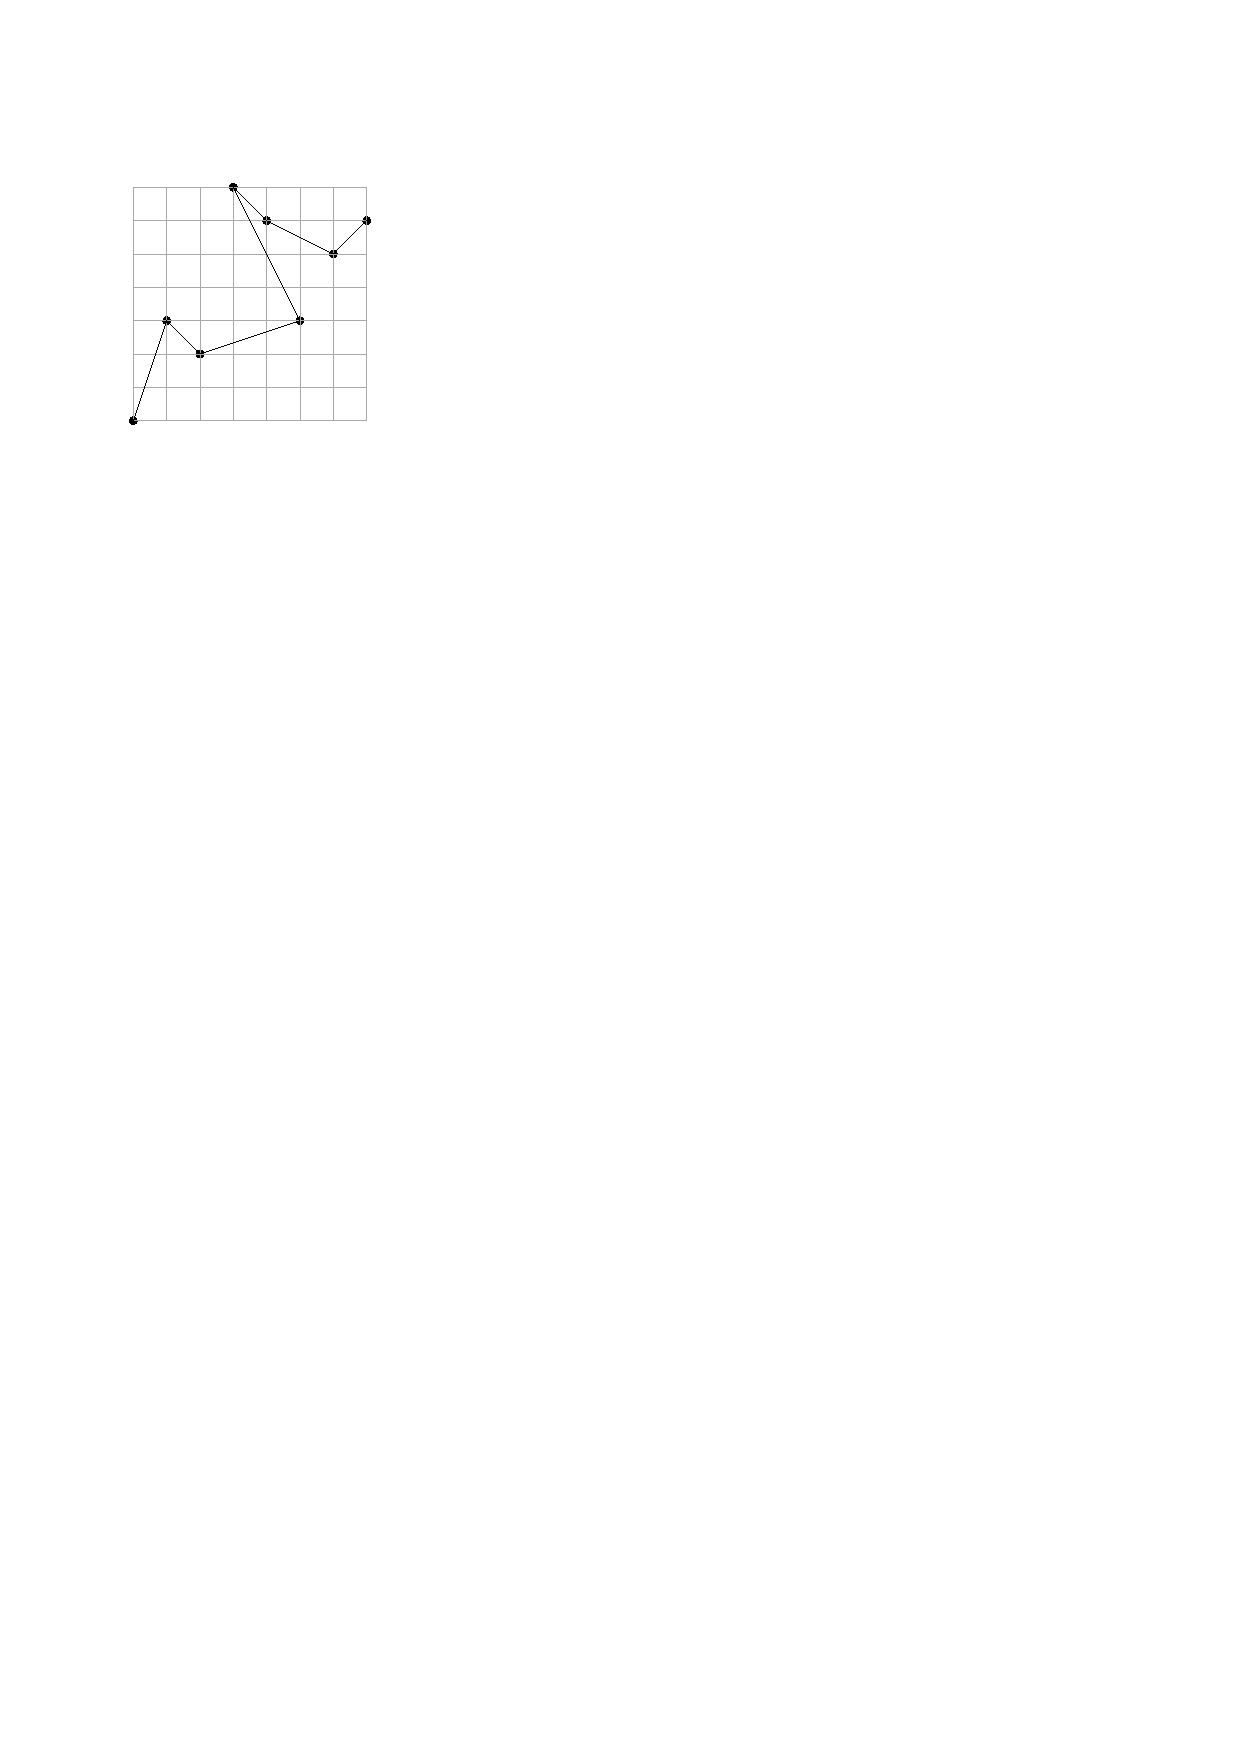
\includegraphics{boxes-perm}
    \caption{The permutation \(\pi_2\) for a pointset in \([8]^2\), listing the
      points with \(y\)-coordinate in \(\{1,2,3,4\}\) first, in
      increasing order of their \(x\)-coordinate, and then listing the
      points with \(y\)-coordinate in \(\{5,6,7,8\}\). The bottom-left
      corner is \((1,1)\).}
    \label{fig:ch2-boxes-perm}
  \end{figure}

  If \(\SS\) is the set system induced by \(\pi_1, \ldots,
  \pi_m\) on \(P\), then, by Theorem~\ref{thm:ch2-kperm},
  \[
  \disc(\SS) \lesssim m \log(2n) \lesssim \log(2n)^2.
  \]
  The theorem is now implied by the bound
  \begin{equation}\label{eq:ch2-tusnady}
    \disc(\AA_d|_P, \col) \le 2(1 + \log_2 n) \disc(\SS, \col),
  \end{equation}
  valid for any coloring $\col$ of $P$.
  Notice that, since we can express any interval of a permutation (i.e., a set
  of the type \(\{\pi(i), \ldots, \pi(j)\}\) for \(i \le j\)) as the
  difference of two prefixes, the discrepancy of any interval of any
  of the permutations \(\pi_k\) is bounded by \(2\disc(\SS,
  \col)\).
  To prove \eqref{eq:ch2-tusnady}, it is then enough show that every anchored box in $\AA_2|_P$ can be written as the disjoint union of $1+\log_2 n$  intervals of the permutations $\pi_1, \ldots, \pi_m$. Take an arbitrary anchored rectangle $\rbox_{0,b} \cap P$. Decomposing its vertical side $[0, b(2)]$ into a disjoint union of canonical intervals allows us to write $\rbox_{0,b}$ as a disjoint union $(\rbox'_1 \cap P) \cup \ldots\cup (\rbox'_\ell\cap P)$ of  $\ell \le 1+\log_2 n$ rectangles, where the vertical side of each $\rbox'_i$ is a canonical interval, and the horizontal side is $[0,b(1)]$. The vertical side of $\rbox'_i$ being a canonical interval implies that all points in $\rbox'_i\cap P$ are listed contiguously in one of the permutations $\pi_k$, i.e., they form an interval of $\pi_k$. This proves our claim, and therefore inequality \eqref{eq:ch2-tusnady} and the theorem.
\end{proof}

\section{Vector Balancing}

Suppose that \(\|\cdot\|_X\) is a norm on \(\R^m\), and recall our
notation for the discrepancy of an \(m\times n\) matrix \(\mat\)
measured in terms of \(\|\cdot\|_X\):
\[
\disc_X(\mat) \eqdef \min_{\col \in \{-1,+1\}^n} \|\mat \col\|_X.
\]
Recall further that the vector balancing constant of a set \(K
\subseteq \R^m\) with respect to the normed space \(X\) is
\[
  \vb(K, X) \eqdef \sup\{\disc_X((u_i)_{i=1}^n): u_1, \ldots, u_n \in
  K, n \in \N\}.
\]

It is natural to set \(K\) to be the unit ball \(B_X = \{u \in \R^m:
\|u\|_X \le 1\}\) of \(X\), and ask how \(\vb(B_X, X)\) can be bounded
in terms of \(m\) and of geometric properties of \(B_X\). The triangle
inequality shows that \(\disc_X(\mat) \le \sum_{i = 1}^n \|u_i\|_X \le
n\) for any matrix \(\mat = (u_i)_{i = 1}^n\) with columns in \(B_X\), 
and this bound holds for \emph{any} coloring \(\col \in \{-1,
+1\}^n\). This bound is weak when \(n\) is much bigger than \(m\), but
the linear algebraic method
allows us to reduce to the
\(n \le m\) case, and show a bound for an arbitrary normed space \(X\)
that only depends on the dimension. 
\begin{theorem}\label{thm:ch2-gen-vb}
  Let \(\|\cdot\|_X\) be a norm on \(\R^m\) with unit ball
  \(B_X\).
  Then \(\vb(B_X, X) \le 2m\), and moreover, for any matrix
  $M$ with columns \(u_1, \ldots, u_n \in B_X\), a
  coloring \(\col\) achieving \(\disc_X(M) \le 2m\) can
  be computed in polynomial time. 
\end{theorem}
\begin{proof}
  %Take some \(u_1, \ldots, u_n \in %B_X\), and define the matrix \(\mat
  %\eqdef (u_i)_{i = 1}^n\).  
  To show that \(\disc_X(\mat) \le
  2m\), by Theorem~\ref{thm:ch2-col-reduction} it suffices to
  show that \(\herdisc_X(\mat,m) \le  m\). The latter follows trivially from the triangle inequality.
\end{proof}

\remark The bound above can be improved to \(\vb(B_X, X) \le m\) by modifying the proof of Theorem~\ref{thm:ch2-col-reduction} in this special case. In particular, rounding the coordinates of the vector $y \in [-1,+1]^J$ in the proof of Theorem~\ref{thm:ch2-col-reduction} to the nearest element of $\{-1,+1\}$, instead of using discrepancy based rounding. We leave the details as an exercise. 

This improvement to Theorem~\ref{thm:ch2-gen-vb} is tight for the \(\ell_1^m\) norm, since
\(\disc_{\ell^m_1}(I) = m\), where \(I\) is the \(m\times m\) identity
matrix. On the other hand, a better bound is possible for every
\(\ell^m_p\) norm when \(p > 1\), as shown in the next theorem. 

\begin{theorem}\label{thm:ch2-ellp-vb}
  Let
  \(B_p^m =\{u\in\R^m:\|u\|_p\le 1\}\) be the unit ball of 
  \(\ell_p^m\). 
  Then,  \(\vb(B_p^m, \ell_p^m) \lesssim m^{1/p},\) for \(1 \le p \le 2\),
  and  \(\vb(B_p^m, \ell_p^m) \lesssim
  \min\{\sqrt{p},\sqrt{\log 2m}\}\sqrt{m}\) for \(p \ge 2\).
\end{theorem}
\begin{proof}
  As in the proof of Theorem~\ref{thm:ch2-gen-vb}, let \(u_1, \ldots,
  u_n \in B_p\), and define the matrix \(\mat \eqdef (u_i)_{i =    1}^n\). 
  By Theorem~\ref{thm:ch2-col-reduction}, it is enough to bound
  \(\herdisc_X(\mat(*,J))\) for any \(J\subseteq [n]\) of size at most
  \(m\), i.e., it suffices to show the discrepancy bounds
  with \(n\) in place of \(m\):
  \begin{align}
    &1 \le p \le 2 \implies \disc_{\ell_p^m}(\mat) \lesssim n^{1/p},\\
    &p \ge 2 \implies \disc_{\ell_p^m}(\mat) \lesssim \min\{\sqrt{p},\sqrt{\log 2m}\}\sqrt{n}.
  \end{align}

  Let us start with the Euclidean case \(p=2\). Then, for \(\col \in \{-1,+1\}^n\)
  chosen uniformly at random, we have the parallelogram law
  \begin{equation}\label{eq:ch2-paralellogram}
    \E\|\mat \col\|_2^2 = 
    \E \Big\|\sum_{i = 1}^n \col(i)u_i\Big\|_2^2 = \sum_{i = 1}^n
    \|u_i\|_2^2 \le n.
  \end{equation}
  So there must then exist at least one coloring \(\col\) such that
  \(\|\mat \col\|_2^2 \le n\), and thus \(\disc_{\ell_2^m}(\mat) \le
  \sqrt{n}\).

  Interestingly, an approximate version of the upper bound in
  \eqref{eq:ch2-paralellogram} holds for any \(p \ge 2\) by the
  type-\(2\) inequality for \(\ell_p\)~\cite[Chapter
  9]{LedouxTalagrand91}. The inequality states that, for a uniformly
  random \(\col \in \{-1,+1\}^n\),
  \begin{equation}\label{eq:ch2-type2}
    \E \Big\|\sum_{i = 1}^n \col(i)u_i\Big\|_p^2 \lesssim {p} \sum_{i = 1}^n
    \|u_i\|_p^2 \le p n.
  \end{equation}
  This implies that, for \(p \ge 2\),
  \(
  \disc_{\ell_p^m}(\mat) \lesssim \sqrt{pn}.
  \)
  
  By the inequalities \(\|x\|_q \le \|x\|_p \le m^{\frac1p -
    \frac1q} \|x\|_q\), which hold for any \(1 \le p \le q \le \infty\), all \(\ell_p^m\) norms are equivalent up to a constant
  for \(p \ge \log m\). Therefore, for \(p \ge \max\{2,\log
  m\}\), we also have the stronger bound
  \(
  \disc_{\ell_p^m}(\mat) \lesssim \sqrt{\log(2m) n}.
  \)
  This takes care of the case \(p \ge 2\).
  
  
  The appropriate analog of the type-2 inequality~\eqref{eq:ch2-type2} for \(1 \le p < 2\) is the type-\(p\) inequality, which states
  that for a uniformly random \(\col \in \{-1,+1\}^n\),
  \[
    \E \Big\|\sum_{i = 1}^n \col(i)u_i\Big\|_p^p \lesssim \sum_{i = 1}^n
    \|u_i\|_p^p \le n.
  \]
  This implies that, for \(1 \le p \le 2\), we have 
  \(
  \disc_{\ell_p^m}(\mat) \lesssim n^{1/p}.
  \)
\end{proof}

% It is possible to derandomize the algorithm in the proof of
% Theorem~\ref{thm:ch2-ell2-vb} to get a polynomial time deterministic
% algorithm achieving the same bound. We omit this derandomization argument here.

The example of the \(m\times m\) identity matrix again shows that the
bounds in Theorem~\ref{thm:ch2-ellp-vb} are tight up to constants for
\(1 \le p \le 2\). The example of an appropriately scaled Hadamard matrix (i.e., an $m\times m$ matrix $M$ with entries in $\{-1,+1\}$ and pairwise orthogonal rows and columns) shows that the bounds are also tight up to the \(\max\{\sqrt{p},\sqrt{\log 2m}\}\)
term for \(p \ge 2\): we leave the details of the argument as an exercise.

As we will see later %\sasho{refer to a specific chapter},
however, a better bound holds for \(p = \infty\) (equivalently, for $p \ge \log m$): this is a landmark result of Spencer (Theorem~\ref{thm:ch3-spencer}), which we prove in Chapter~\ref{ch:partial}.


Let us finally remark that the proof of the Beck-Fiala theorem
(Theorem~\ref{thm:ch2-bf}) can be generalized to show that \(\vb(B_1^m,
\ell_\infty^m) \le 2\). We leave this generalization as an
exercise. 

We recall here the  Koml\'os problem
(Problem~\ref{prob:komlos} from the Introduction), asking to determine
if \(\vb(B_2^m, \ell_\infty^m) \lesssim 1\). A positive resolution of this problem also implies a
positive resolution of the Beck-Fiala conjecture mentioned earlier.
In general, it is an interesting problem to determine how the vector
balancing constant \(\vb(B_p^m, \ell_q^m)\) depends on \(m\) when
\(p\) is much smaller than \(q\).

\section{Prefix Discrepancy and Signed Series}

Next, we recall the Steinitz problem, where given \(n\) ``short''
vectors \(u_1, \ldots, u_n \in \R^m\) whose sum is \(0\), we ask
if the vectors can be rearranged so that all partial sums are
bounded independently of \(n\). As we saw in the Introduction, the Steinitz problem is closely related to the
prefix discrepancy of a matrix \(M = (u_i)_{i = 1}^n\), defined as
\[
  \pdisc_X(M) \eqdef \min_{\col \in \{-1, +1\}^n}
  \max_{j=1}^n \Big\|\sum_{i = 1}^j \col(i) u_i\Big\|_X,
\]
where \(\|\cdot\|_X\) is a norm. Namely, by
Theorem~\ref{thm:ch1-chobanyan} (Chobanyan's transference theorem), 
the Steinitz
constant of \(M = (u_i)_{i = 1}^n\), 
\[
  \st_X(M) = \min_{\pi \in S_n} \max_{j = 1}^n \Big\|\sum_{i = 1}^j
     u_i - \frac{j}{n} \sum_{k = 1}^n u_k\Big\|_X,
\]
satisfies the bound
\[
  \st_X(M) \le \max_{\pi \in S_n}\pdisc_X(\pi \circ M),
\]
where \(\pi \circ M \eqdef (u_{\pi(i)})_{i = 1}^n\) is the rearrangement of
the columns of \(M\) according to \(\pi\). In other words, the
worst-case prefix discrepancy over re-arrangements of the columns of
\(M\) bounds the Steinitz constant.

Let us recall the notation for the worst-case Steinitz constant
and the worst-case prefix discrepancy: for a set \(K
\subseteq \R^m\), and a normed space \(X = (\R^m,\|\cdot\|_X)\), we  have
\begin{align*}
  &\st(K, X) \eqdef \sup\{\st_X((u_i)_{i=1}^n): u_1, \ldots, u_n \in K, n \in \N\},\\
  &\sser(K, X) \eqdef \sup\{\pdisc_X((u_i)_{i=1}^n): u_1, \ldots, u_n \in K, n \in \N\}.
\end{align*}
Chobanyan's lemma then implies that \(\st(K,X) \le \sser(K,X)\) for any
\(K\) and \(X\). %Therefore, if we formalize the Steinitz problem as
%asking us to show that \(\st(B_X, X)\) is bounded by a function only
%of the dimension \(m\), it is enough to show such a bound on
%\(\sser(B_X, X)\), instead. We do so 
The next theorem bounds these by $2m$.
This significantly strengthens Theorem~\ref{thm:ch2-gen-vb}, by extending the bound there for discrepancy to that for prefix discrepancy.

\begin{theorem}\label{thm:ch2-gen-st}
  Let \(\|\cdot\|_X\) be a norm on \(\R^m\) with unit ball
  \(B_X\).
  Then
  \[
    \st(B_X, X) \le \sser(B_X, X) \le 2m.
  \]
  Moreover, for any matrix \(M\) with columns \(u_1, \ldots, u_n \in B_X\), a
  coloring \(\col\) achieving \(\pdisc_X(M) \le 2m\) can
  be computed in polynomial time. 
\end{theorem}

\paragraph{The Algorithm.} We use our template via Lemma~\ref{lm:ch2-linalg-gen}. However, unlike previous examples, we will choose the active coordinates \(\act\) more carefully (among the coordinates that have not yet reached \(+1\) or \(-1\)). 
Also, we can assume that \(m < n\),
otherwise the theorem holds trivially for any arbitrary coloring by the triangle inequality for \(\|\cdot\|_X\).


As usual, let $\col_{t-1}$ be the coloring at the  beginning of step $t$, and 
initially, \(\col_0 \eqdef
  0\).  At each step \(t
  \ge 1,\) we choose \(\act_{t}\) to consist of the first \(m+1\) indices
  \(i_1, \ldots, i_{m+1}\) satisfying \(|\col_{t-1}(i_j)|<1\) for all
  \(j \in [m+1]\). In particular, at $t=1$, \(\act_1 \eqdef [m+1]\). 
In other words, $A_t$ can be viewed as a sliding window of the first $m+1$ strictly fractional coordinates.  
At step $t$, applying Lemma~\ref{lm:ch2-linalg-gen} to \(\mat\),
  \(\col_{t-1}, A_t \)
  gives a fractional coloring
  \(\col_{t}\) such that
  \begin{enumerate}
  \item \(\mat \col_t = \mat x_{t-1}\);
  \item for all \(i \in [n]\setminus\act_{t}\), \(\col_t(i) = \col_{t-1}(i)\);
  \item at least one element \(i \in \act_{t}\) satisfies
    \(|\col_t(i)| = 1\).
  \end{enumerate}

We terminate whenever fewer
than \(m+1\) such indices are left -- once that happens,
  say at step \(T\), we set \(\col(i) \eqdef \col_T(i)\) whenever
  \(|\col_T(i)| = 1\), and otherwise we set \(\col(i)\) arbitrarily, and output $\col$.

\paragraph{Analysis.} As the rank of \(\mat(*,\act_{t})\) is at most \(m < |\act_{t}| = m+1\), at each step $t$, at least one variable in $A_t$ reaches $\pm 1$, and the algorithm terminates in at most $n$ steps.

To analyze the (prefix) discrepancy, let us fix some arbitrary \(j \in [n]\), and track how the discrepancy 
$d_t = \|\sum_{i=1}^j x_t(i) u_i \|_X$ evolves over time. Clearly, $d_0=0$ as each $x_0(i)=0$ initially.
The key observation is that as long as $A_t \subseteq [j]$, i.e., the sliding window $A_t$ is contained in the first $j$ coordinates, the discrepancy $d_t$ of this prefix stays zero.

To see this, let $\max(\act_t)$ denote the largest coordinate in $\act_t$, and let $t_j$ be the last time step when
  \( \max(\act_t)\leq j\).   
  % A key claim in the
  % proof is that
  % \begin{equation}\label{eq:ch2-ss-zero}
  % \sum_{i=1}^j \col_t(i) u_i = 0.
  % \end{equation}
  As \(\max (\act_s)\) is non-decreasing in $s$ by our choice of
  \(\act_s\), we have that, for all \(1 \le s \le t_j\), \(\act_{s} \subseteq
  [j]\). Since the colorings \(\col_s\) and \(\col_{s-1}\) are equal
  outside \(\act_{s}\),
  \[
    \sum_{i=1}^j (\col_s(i) - \col_{s-1}(i))u_i =  \mat (\col_s -
    \col_{s-1}) = 0,
  \]
  and thus $d_{s}-d_{s-1} = 0$.
  Adding up these equalities over \(s \in [t_j]\), and using
  \(d_0 = 0\) yields $d_{t_j}=0$. 

  To finish the analysis, notice that the final coloring \(\col\) can differ 
  from the coloring
  \(\col_{t_j}\)
  in at most \(m\) coordinates in
  \([j]\). This is because for any coordinate \(i \le j\),  \(\col(i)\) can differ from  \(\col_{t_j}(i)\)
  only if \(i \in \act_{t_j+1} \cap [j]\), and there are only
  \(m\) such \(i\) by our choice of $t_j$.
  As \(|\col(i) -\col_{t_j}(i)|\leq 2\) for any such $i$ and $\|u_i\|_X\leq 1$,  by the triangle inequality we have that $d_t \leq 2m$. This completes the analysis of the algorithm.
  
  % We can now calculate
  % \begin{align}
  %   \left\|\sum_{i=1}^j \col(i) u_i\right\|_X
  %   &\le     \left\|\sum_{i=1}^j \col_t(i) u_i\right\|_X +
  %   \left\|\sum_{i=1}^j (\col(i)-\col_t(i)) u_i\right\|_X\label{eq:ch2-ss-tri1}\\
  %   &=  \left\|\sum_{i\in \act_t \cap [j]} (\col(i)-\col_t(i)) u_i\right\|_X\label{eq:ch2-ss-diff}\\
  %   &\le \sum_{i \in \act_t \cap [j]} |\col(i) - \col_t(i)|\|u_i\|_X\label{eq:ch2-ss-tri2}\\
  %   &< 2|\act_t\cap [j]| \le 2m.\label{eq:ch2-ss-final}
  % \end{align}
  % Above, \eqref{eq:ch2-ss-tri1} and \eqref{eq:ch2-ss-tri2} follow from
  % the triangle inequality, \eqref{eq:ch2-ss-diff} follows from
  % \eqref{eq:ch2-ss-zero}, and the final inequality
  % \eqref{eq:ch2-ss-final} holds because, for all \(i\), \(\col(i) - \col_t(i) \in (-2,
  % 2)\), \(\|u_i\|_X \le 1\) by
  % assumption, and \(|\act_t\cap [j]| \le m\), as we established in the
  % previous paragraph. 

\remark
This bound can be slightly improved to \(\sser(B_X, X)\le 2m-1\), by optimizing the proof above further.
For $\st(B_X, X)$, a bound of \(\st(B_X, X) \le m\) can also be shown for all
normed spaces \(X\) using a different linear algebraic argument. Both bounds are tight up to a constant factor for \(X =
\ell_1^m\). 

Recall the conjecture from the introduction that both bounds can be improved to
\(O(\sqrt{m})\) for \(X = \ell_2^m\) and \(X = \ell_\infty^m\). We remark that
there is \emph{no \(m\)-dimensional normed space}, let alone these
two, for which a bound that is asymptotically better than \(O(m)\) has been shown. 
%We will return to to the following problem later in this
% book.
% \begin{problem}
%   Give tight bounds on the quantities \(\st(B_p^m,\ell_p^m),
%   \sser(B_p^m,\ell_p^m)\) in terms of \(m\) for \(p \in \{2,
%   \infty\}\), or, more generally, for \(p > 1\). 
% \end{problem}

\section{Bibliographic Notes}

Theorem~\ref{thm:ch2-bf} is due to Beck and Fiala~\cite{BF81}, who
also pioneered the linear algebraic method presented in this
chapter. Exercise~\ref{ex:ch2-bf-improvement} is due to Bednarchak and
Helm~\cite{BH97-beckfiala}. The best known upper bound on discrepancy purely in terms of
the degree is $2\ssdeg(\SS) - \log^*(\ssdeg(\SS))$ and is due to
Bukh~\cite{Bukh16}. Very recently, Bansal and Jiang showed an $O(\sqrt{\ssdeg(\SS)})$ bound whenever $\ssdeg(\SS) = \Omega(\log^2n)$. For general $\ssdeg(\SS)$, they obtain an $\widetilde{O}(\sqrt{\ssdeg(\SS)} + \sqrt{\log n})$ bound, where $\widetilde{O}(\cdot)$ hides factors polynomial in $\log \log n$.
Their techniques also give an $O(\log^{1/4} m)$ discrepancy bound for the Koml\'{o}s problem.
%building on the techniques we will see in Chapter \ref{ch:algo-komlos-bana}. However, we will not discuss their result in this book.


The application of the Beck-Fiala theorem to the discrepancy of
axis-aligned boxes in Theorem~\ref{thm:ch2-bftusnady} is due
to Beck~\cite{beck-rect}. Theorems~\ref{thm:ch2-kperm}~and~\ref{thm:ch2-tusnady} are due to
Bohus~\cite{Bohus}. Beck asked whether the $\log n$ term can be
removed in Theorem~\ref{thm:ch2-kperm} for $3$ (or more)
permutations. He also proved that the discrepancy of $2$ permutations
is at most $1$: see~\cite{spencer-lectures}. Newman, Neiman, and Nikolov
answered Beck's question negatively and showed that the $O(\log n)$ bound is
tight for $3$ permutations~\cite{beck3perm}. Franks gave a simplified proof of this
result~\cite{Franks21}.  While the dependence on $n$ in
Theorem~\ref{thm:ch2-kperm} is tight, it is possible to improve the
dependence on $k$~\cite{SST-perms}, as we will see in the next
chapter. An upper bound on the discrepancy of $k$ permutations that is
simultaneously tight in terms of both $k$ and $n$ is not known.

Theorems~\ref{thm:ch2-gen-vb}~and~\ref{thm:ch2-gen-st}
are due to B\'ar\'any and Grinberg~\cite{baranygrinberg}. 
Sevastjanov, and Sevastjanov and Grinberg used linear algebraic
arguments to give better bounds for the Steinitz constant, showing
that it is bounded by $d$ in any $d$-dimensional normed
space~\cite{Sev78,GS80}. Their proof develops a linear algebraic
argument directly for the Steinitz problem, rather than going through
discrepancy, and gives a better bound than
Theorem~\ref{thm:ch2-gen-st}. This argument, and more applications of
linear algebraic methods to vector balancing and related problems can
be found in B\'ar\'any's survey~\cite{B08}. 

Linear algebraic arguments similar to the ones in this chapter have
also found applications in the design of approximation algorithms for
computationally hard problems. An early example is the work of
Karmarkar and Karp on the bin packing
problem~\cite{KarmarkarK82}. Many more algorithms using these
techniques are surveyed by Lau, Ravi, and
Singh~\cite{iterative-book}. 

%%% Local Variables:
%%% mode: latex
%%% TeX-master: "book"
%%% End:
